% Created 2014-04-04 Fri 19:09
\documentclass{article}
\usepackage[utf8]{inputenc}
\usepackage[T1]{fontenc}
\usepackage{fixltx2e}
\usepackage{graphicx}
\usepackage{longtable}
\usepackage{float}
\usepackage{wrapfig}
\usepackage{soul}
\usepackage{textcomp}
\usepackage{marvosym}
\usepackage{wasysym}
\usepackage{latexsym}
\usepackage{amssymb}
\usepackage{hyperref}
\usepackage{tikz}
\usepackage{color}
\usepackage{listings}


\graphicspath{ {images/} }

\tolerance=1000
\providecommand{\alert}[1]{\textbf{#1}}

\title{Synchronization in Linux}
\author{Aakarsh Nair}
\date{\today}

\begin{document}

\lstdefinestyle{customc}{
%  basicstyle=\footnotesize,       % the size of the fonts that are used for the code
  numbers=right,                   % where to put the line-numbers
  numberstyle=\footnotesize,      % the size of the fonts that are used for the line-numbers
  stepnumber=1,                   % the step between two line-numbers. If it is 1 each line will be numbered
  numbersep=5pt,                  % how far the line-numbers are from the code
  backgroundcolor=\color{white},  % choose the background color. You must add \usepackage{color}
  showspaces=false,               % show spaces adding particular underscores
  showstringspaces=false,         % underline spaces within strings
  showtabs=false,                 % show tabs within strings adding particular underscores
  frame=single,           % adds a frame around the code
  tabsize=2,          % sets default tabsize to 2 spaces
  captionpos=b,           % sets the caption-position to bottom
  breaklines=true,        % sets automatic line breaking
  breakatwhitespace=false,    % sets if automatic breaks should only happen at whitespace
  escapeinside={\%*}{*)},          % if you want to add a comment within your code
  %% belowcaptionskip=1\baselineskip,
  %% breaklines=true,
  %% frame=L,
  %% xleftmargin=\parindent,
  language=C,
  %% showstringspaces=false,
  basicstyle=\footnotesize\ttfamily,
  keywordstyle=\bfseries\color{green!40!black},
  commentstyle=\itshape\color{purple!40!black},
  %% identifierstyle=\color{black},
  stringstyle=\color{orange},
}

\lstdefinelanguage{anX86} {
	morekeywords={
		nop,movl,pushl,popl,cmpl,testl,leal,cmovl,jmp,je,jne,
		jz,jnz,jg,jge,jl,jle,addl,subl,imul,idiv,cdq,incl,decl,
		negl,andl,orl,xorl,notl,shrl,shll,sarl,sall,ret,leave,
		call,setg,setl,setge,setle,setne,sete,movzbl,
		eax,ebx,ecx,edx,edi,esi,ebp,esp,al,bl,cl,dl,
                pause,lock,decb,jns,jle,jmp,cmpb,movb,xchg,xchgb,lea
	},
	sensitive=true,
	morecomment=[l]{\#},
	morestring=[b]"
}
\lstset{escapechar=@,style=customc}
\lstset{language=C}

\maketitle

\setcounter{tocdepth}{3}
\tableofcontents

\maketitle
\vspace*{1cm}

\section{Introduction}

Synchronization becomes necessary when the outcome of a computation
depends on how two or more interleaved kernel control paths are
nested. Critical regions are parts of code that must be executed by at
most one kernel control path to completion before another kernel
control path is allowed to execute it.


\section{Kernel Preemption}

Process running in Kernel Mode can be replaced by another process.
The main reason for making a kernel preemptive is to reduce the
dispatch latency of user mode processes (the time between when they
become runnable and begin running).  Process switches happens via
the\lstinline{switch_to_macro}.

Kernel premption is enabled and disabled via the
\lstinline{prempt_count} in the \lstinline{thread_info}. A task is
premptible if \lstinline{thread_info()->preempt_count} is zero.

The \lstinline{prempt_count} is greater than zero if 

\begin{itemize}
\item The kernel is executing in an interrupt service routine.
\item kernel is executing a tasklet of a softirq
\item kernel preemption has been explicitly disabled setting it to a
  positive value
\end{itemize}


The \lstinline{prempt_count} is an amalgamation of three separate
counters meant to keep track number of times kernel preemption count
as well as softirq and hardirq counts.

\begin{center}
  \begin{tabular}{| l | l | }    
    \hline
    Bits & Description                    \\ \hline
    0-7 & Preemption counter (max=255)    \\ 
    8-15 & Softirq counter (max=255)      \\ 
    16-27 &  Hardirq counter (max=4096)   \\ 
    28 & \lstinline{PREEMPT_ACTIVE} flag  \\ \hline
  \end{tabular}
\end{center}

Thus kernel is preempted only when its executing an exception handler
and kernel preemption has not been explicitly disabled and the local
CPU has local interrupts enabled.

Key Macors Dealing with preemption counter are given as 

\begin{center}
  \begin{tabular}{| l | p{9 cm} |}    
    \hline
    Bits & Description                    \\ \hline
    \lstinline{preempt_count()} & Select the \lstinline{preempt count} from \lstinline{thread_info}    \\ 
    \lstinline{preempt_disable()} & Increase the value of the preemption counter.     \\ 
    \lstinline{preempt_enable_no_resched()} &  Decrease by one the value of the preemption counter  \\
    \lstinline{preempt_enable()} & Decrease by one the value of preemption counter and call \lstinline{preempt_schedule()} if \lstinline{TIF_NEED_RESCHED} on \lstinline{thread_info} is set \\
    \lstinline{get_cpu()} & Similar to \lstinline{preempt_disable()} but also returns the number of local CPU \\
    \lstinline{put_cpu()} & Same as  \lstinline{preempt_enable()} \\
    \lstinline{put_cpu_no_resched()} & Same as \lstinline{preempt_enable_no_resched()}    \\
    \hline
  \end{tabular}
\end{center}


\section{Kernel Synchronization Primitives}

The linux kernel provides several synchronization primitives these
include

\begin{itemize}
\item \textbf{Per-CPU variables}
  Use duplicate data structures for each CPU
\item \textbf{Atomic Operations}
  Atomically read-modify-write instruction to a counter
\item \textbf{Memory Barrier}
  Avoid instruction reordering
\item  \textbf{Spinlock}
  Lock with a busy wait
\item \textbf{Semaphores}
  Lock with blocking wait/sleep.
\item \textbf{Seqlocks}
  Lock based on access counter
\item \textbf{Local interrupt disabling}
  Forbid interrupt handling on a single CPU
\item \textbf{Local softirq disabling}
  Forbid deferrable function handling on a single CPU
\item \textbf{Read Copy Update}
  Lock free access to shared data structures using pointers
\end{itemize}

Many of these synchronization constructs depend on implementation of
atomic operations implemented at the chip level on CPUs. Thus are
specific to the architecture they are executing on.

\subsection{Processor guarantees}

\begin{itemize}
  \item On a particular CPU dependent memory accesses happen in order
    of issuance.

  \item Overlapping loads and stores within a particular CPU will
    appear to be ordered within a CPU
    
\end{itemize}

Things which cannot be assumed

\begin{itemize}
\item it \textbf{must not} be assumed that compilers will not reorder
  memory references not protected with \lstinline{ACCESS_ONCE()}. Without
  \lstinline{ACCESS_ONCE()} the compiler can perform transformations see memory
  barriers.
\item it \textbf{must not} be assumed that independent loads and
  stored will be issued in any given order.
\item it \textbf{must not} be assumed that overlapping memory accesses
  may be merged or discarded.  
\end{itemize}

Things that we anti-guarantees (bad stuff will happen):

\begin{itemize}

\item Compilers will often generate code to modify bit fields using non
  atomic read-modify write sequences

\item All fields in a given bit-field must be must be protected by one
  lock. Update of one field can be corrupted by another by compiler.
  
\item Guarantees only apply to properly aligned and sized scalar
  variables. Same size as "char","short","int" and "long".  
\end{itemize}

\subsection{Memory Barrier}

Memory barriers impose perceived partial ordering over memory
operations on either side of the barrier.

Memory barriers provide a way to instruct the compiler and CPU to
restrict the order in which instructions are executed. Performance
optimizations of compilers and CPUs play havoc with synchronization
primitives. These include compiler reordering instructions to optimize
register usage, CPUs executing instructions in parallel, reordering
memory accesses.


Types of performance tricks memory barriers may protect against are
\begin{itemize}
\item Reordering and deferral of combination of memory operations
\item Speculative loads
\item Speculative branch prediction and caching
\end{itemize}

Memory barrier types include

\begin{itemize}
\item Write (or store) memory barrier

  A write memory barrier gives guarantee that all STORE operations
  specified before the barrier will happen before all STORE operations
  STORE operations specified after the barrier. wrt. other components
  in the system.

  A partial order on STORES only. Does not affect LOADS.

  CPU can be viewed as performing a commit. All stores before the
  write barrier will occur before all stores after the write barrier.

  Should not be paired with read or data dependency barrier.
  
\item Data dependency barrier

  Weaker form of read barrier. Two loads such that the second depends
  on result of first ( first load retrieves the address which to which
  second load is directed). Ensure the target of second load is
  updated before first load accessed %% (??)

  Partial ordering on inter-dependent loads only. No effect on
  independent loads or overlapping loads. Has no affect on stores.

  A data dependency barrier issued by the CPU is thus a line in the
  sand such that for any loads preceding it, if that load touches one
  of a sequence of stores from another CPU then by the time the
  barrier completes(the line is crossed) the effect of all stores
  prior to that load will be perceptible by any loads issued after the
  data dependency barrier.

  Thus a dependency barrier is an optimization to prevent the
  requirement for a full read (or load) barrier.


\item Read (or load) memory barrier

  A read load barrier is a data dependency barrier plus a guarantee
  that all LOAD operations specified before the barrier will appear to
  happen before all the LOAD operations specified after the barrier
  wrt other components in the system.

  A partial ordering on loads only; no required effect on stores.

  Imply data dependency barrier.

  Should be paired with write barriers %%??

  
  
\item General Memory barrier

  All LOAD and STORE operations before the barrier will happen before
  all LOAD and STORE operations specified after the barrier with
  respect to other components of the system.

  A partial ordering over both loads and stores.  

\item Implicit Barriers
  \begin{itemize}
  \item ACQUIRE operations
  \item RELEASE operations
  \end{itemize}
\end{itemize}


\subsection{Data Dependency Barrier}

To better understand need for data dependency barriers consider 
the following sequence of instructions:

\begin{lstlisting}
	CPU 1		      CPU 2
	===============	      ===============
	{ A == 1, B == 2, C = 3, P == &A, Q == &C }
	B = 4;
	<write barrier>
	ACCESS_ONCE(P) = &B
			      Q = ACCESS_ONCE(P);
			      D = *Q;
\end{lstlisting}

While the write barrier will guarantee that all writes seen by both
processors.  After the barrier Q will be assigned either the address
of B or the address of A depending on whether the update to P was seen
by CPU2 or not.

D is assigned a dereference to Q. We thus expect the dereference to
dereference A or B getting values of A=1 or B=4.

BUT, CPU 2's perception of P may be updated before its perception of B
leading to the following situation.

\begin{lstlisting}
(Q = &B) and (D = 2 ) 
\end{lstlisting}
%% ???

\begin{lstlisting}
        CPU 1		      CPU 2
	===============	      ===============
	{ A == 1, B == 2, C = 3, P == &A, Q == &C }
	B = 4;
	<write barrier>
	ACCESS_ONCE(P) = &B
			      Q = ACCESS_ONCE(P);
			      <data dependency barrier>
			      D = *Q;  
\end{lstlisting}

The data dependency barrier forces the assignment of B to show up on
processor 2 when Q is assigned a pointer to B.

%% \subsubsection{Multiple Reads}

\subsection{Control Dependencies}

Control dependencies are those which require a full read memory
barrier where a data dependency barrier will simply not suffice.

\begin{lstlisting}
q = ACCESS_ONCE(a);
if (q) {
  <data dependency barrier>  /* BUG: No data dependency!!! */
  p = ACCESS_ONCE(b);
}
\end{lstlisting}

Here CPU may attempt to short circuit in an attempt to predict the
branch outcome. Thus the load from b may appear to happen before the
load from a.

The solution for this is to impose a read barrier to ensure that b is
read


While LOAD is speculated the STORES are NOT speculated. Thus the
ordering semantics of following will not be affected.

\begin{lstlisting}
  q = ACCESS_ONCE(a);
  if (q) {
    ACCESS_ONCE(b) = p;
  }  
\end{lstlisting}


The \lstinline{ACCESS_ONCE} directive is aimed at the compiler to
prevent it from merging separate loads from 'a' and separate stores to
'b'.

TODO ......

%% \subsection{SMP Barrier Pairing}
%% \subsection{Read Memory Barriers vs Load Speculation}
%% \subsection{Transitivity}

\subsection{Explicit Kernel Barriers}

\subsubsection{Compiler Barriers}

Used primarily to prevent the compiler from reordering instructions
the \lstinline{barrier()} is a general barrier. The
\lstinline{ACCESS_ONCE()} macro is a weaker form of the barrier
instruction which only affects instructions flagged by
\lstinline{ACCESS_ONCE()}.

Can be implemented using the

\lstinline{barrier()} macro expanding to \lstinline{asm volatile"":::memory}

Tells the compiler to insert empty assembly fragment. While the
volatile keyword forbids the compiler from shuffling the instruction.
The memory keyword forces the compiler to use memory locations instead
of those stored in the register. The CPU can still mix assembly
instruction

Effects of \lstinline{barrier()}:

\begin{itemize}
  \item Prevent compiler from reordering accesses following barrier()
    with those preceding them them.

  \item Within loop, foce compiler to lad variables used in loop
    conditional on each pass through loop.    
\end{itemize}

Effects of \lstinline{ACCESS_ONCE()} , prevent optimizations that
though safe in single threaded code will break concurrent code.


\begin{itemize}
\item Provide cache coherence for accesses from multiple CPUs to
  single variable. Prevent compiler for reordering loads and stores to
  same variable.
  
  Thus
  \begin{lstlisting}
    a[0] = ACCESS_ONCE(x);
    a[1] = ACCESS_ONCE(x);
  \end{lstlisting}
  Will prevent \lstinline{a[1]} from receiving older value of x than
  \lstinline{a[0]}.

\item Prevent merging successive loads

  \begin{lstlisting}
    while (tmp = ACCESS_ONCE(a))
		do_something_with(tmp);
  \end{lstlisting}

  Will prevent the compiler from optimizing the loop otherwise as

  \begin{lstlisting}    
	if (tmp = a)
		for (;;)
			do_something_with(tmp);
  \end{lstlisting}

\item 
  
\item
\end{itemize}

It is not necessary to use \lstinline{ACCESS_ONCE()} on variables
marked volatile since it is implemented as a volatile cast.

It must be noted that compiler barriers \textbf{\emph{DO NOT}}
directly affect the CPU, which may still reorder instructions.


\subsubsection{CPU Memory Barriers}

All memory barriers except data dependency barriers imply compiler
barrier. SMP memory barriers are reduced to compiler barriers on
uni-processor compiled systems. All memory barriers except data
dependency barriers imply a compiler barrier.

\begin{center}
  \begin{tabular}{| l| l | l | }    
    \hline
    Type & Mandatory & SMP Conditional \\ \hline
    GENERAL & \lstinline{mb()} & \lstinline{smb_mb()} \\ 
    WRITE & \lstinline{wmb()} & \lstinline{smp_wmb()}  \\ 
    READ &  \lstinline{rmb()} & \lstinline{smp_rmb()}  \\
    DATA DEPENDENCY &  \lstinline{read_barrier_depends()} & \lstinline{smp_read_barrier_depends()} \\
    \hline
  \end{tabular}
\end{center}


\subsubsection{Memory barrier and 80x86}

  In 80x86 list of serializing instructions which act as memory
  barriers:


  \begin{itemize}
    \item I/O port operations
    \item instructions with lock byte
    \item instructions affecting the IF flag in eflags register such as those instructions which write to registers
      \begin{itemize}
        \item control registers (cli)
        \item system  registers (sti)
        \item debug   registers          
      \end {itemize}
    \item Some instructions introduced in Pentium 4
      \begin{itemize}
        \item lfence - read barriers
        \item sfence - write barries
        \item mfence - read write barriers
      \end{itemize}
    \item Speial instructions - iret terminating interrupt or exception handler                  
  \end{itemize}
  
%%\end{itemize}

Read barriers maintain the serial order of read instructions, write
barriers maintain serial order of write instructions.

\begin{center}
  \begin{tabular}{| l | l | }    
    \hline
    Function/Macors & Description \\ \hline
    \lstinline{mb()} & Memory barrier for MP and UP \\ 
    \lstinline{rmb()} & Read memory barrier for MP and UP  \\ 
    \lstinline{wmb()} &  Write memory barrier for MP and UP \\
    \lstinline{smp_mb()} &  Memory barrier for MP only \\
    \lstinline{smp_rmb()} &  Read memory barrier for MP only \\
    \lstinline{smp_wmb()} &  Write memory barrier for MP only \\
    \hline
  \end{tabular}
\end{center}
  Macro expansions on  80x86

\begin{center} 
  \begin{tabular}{ | l | p{9 cm} | }    
    \hline
    Function/Macors & Description \\ \hline
    mb() & \lstinline{asm volatile("mfence":::"memory")}  \\  \hline
    rmb() &
\begin{lstlisting}
  asm volatile ("lfence")
  or
  asm volatile ("lock;addl 0,0(%esp)":::"memory")
\end{lstlisting}
      \\ \hline
      \lstinline{wmb()} & \lstinline{barrier()}
      Intel never reorders write memory access so we get only a compiler barrier here.  \\ \hline
    \lstinline{smp_mb()}  & \lstinline{mb()}   \\ \hline
    \lstinline{smp_rmb()} &  \lstinline{barrier()} or \lstinline{rmb()} depending on \lstinline{CONFIG_X86_PPRO_FENCE}\\ \hline
    \lstinline{smp_wmb()} & \lstinline{barrier()} \\     \hline
  \end{tabular}
\end{center}


%% The usage of mandatory barrier may be used to control MMIO effects
%% since they affect the order in which memory operations appear to
%% device and prevent the compiler and CPU from reordering them.


\subsection{Implicit Kernel Memory Barriers}

Many locking and scheduling functions imply memory barriers. We
consider the some of these implicit barriers.

\subsubsection{Acquiring Functions}

Following are examples of acquiring functions inside the kernel.

\begin{itemize}
  \item Spin Locks
  \item Read/Write Spin locks
  \item Mutexes
  \item Semaphores
  \item Read/Write Semaphores
  \item RCU
\end{itemize}

\begin{itemize}
  
\item \textbf{ACQUIRE Implication} \\

  Post-ACQUIRE operations \emph{will be completed} after after ACQUIRE
  completion.

  Pre-ACQUIRE operations \emph{may be completed} after ACQUIRE
  completion.
  
\item \textbf{RELEASE Implications} \\

  Pre-RELEASE operations \emph{will be completed} before RELEASE
  completion.

  Post-RELEASE operations \emph{may be completed} before RELEASE
  completion.

\item \textbf{ACQUIRE vs ACQUIRE Implication} \\

  All ACQUIRE operations will be completed before successive ACQUIRE
  operation .

\item \textbf{ACQUIRE vs RELEASE Implication} \\

  All ACQUIRE operations issued before RELEASE operation will be
  completed before RElEASe operation.

\item \textbf{Failed conditional ACQUIRE Implication} \\

  Failed lock operations don't imply any barrier.
  
\end{itemize}

%% Due to the possibility that pre-ACQUIRE operations may happen after
%% ACQUIRE and post-RELEASE may happen before RELEASE thus accesses may
%% cross.

%% \begin{lstlisting}
%%   *A = a;
%%   ACQUIRE M
%%   RELEASE M
%%   *B = b;
%% \end{lstlisting}

%% May get run as

%% \begin{lstlisting}
%%   ACQUIRE M, STORE *B, STORE *A, RELEASE M
%% \end{lstlisting}

%% Also RELEASE followed by ACQUIRE does not imply a full memory barrier.

%% \begin{lstlisting}  
%% 	*A = a;
%% 	RELEASE M
%% 	ACQUIRE N
%% 	*B = b;
%% \end{lstlisting}

%% May run as :


%% \begin{lstlisting}
%%   ACQUIRE N, STORE *B, STORE *A, RELEASE M
%% \end{lstlisting}



\subsubsection{Interrupt Disabling Functions}
Functions disabling/enabling interrupts will only act as compiler
barriers. 

%% \subsubsection{Sleep and Wake up Functions}
%% \subsubsection{Miscellaneous Functions}

\subsection{Atomic Operations}

Many atomic operations imply full memory barriers and are heavily
relied upon in the kernel.

Any atomic operation that modifies state in memory and returns
information about the state implies SMP-conditional memory barrier.
on each side of the operation. That is \lstinline{smp_mb()}.

Some atomic operations that imply SMP general memory barrier are given
in the table.

\begin{center}
  \begin{tabular}{| l | l |}    
    \hline
    Atomic Operations &  \\ \hline
    \lstinline{xchg()}; & \\
    \lstinline{cmpxchg()}; & \\
    \lstinline{atomic_xchg()}; &			\lstinline{atomic_long_xchg()} \\
    \lstinline{atomic_cmpxchg()}; &		        \lstinline{atomic_long_cmpxchg()} \\
    \lstinline{atomic_inc_return()}; &		        \lstinline{atomic_long_inc_return()} \\
    \lstinline{atomic_dec_return()}; &		        \lstinline{atomic_long_dec_return()} \\
    \lstinline{atomic_add_return()}; &		        \lstinline{atomic_long_add_return()} \\
    \lstinline{atomic_sub_return()}; &		        \lstinline{atomic_long_sub_return()} \\
    \lstinline{atomic_inc_and_test()}; &		\lstinline{atomic_long_inc_and_test()} \\
    \lstinline{atomic_dec_and_test()}; &		\lstinline{atomic_long_dec_and_test()} \\
    \lstinline{atomic_sub_and_test()}; &		\lstinline{atomic_long_sub_and_test()} \\
    \lstinline{atomic_add_negative()}; &		\lstinline{atomic_long_add_negative()} \\
    \lstinline{test_and_set_bit()}; & \\
    \lstinline{test_and_clear_bit()}; & \\
    \lstinline{test_and_change_bit()}; &     \\
    \hline
  \end{tabular}
\end{center}

These operations of often used for implementing ACQUIRE and RELEASE
operations and maintaining reference counters.


\subsubsection{Atomic Operations 80x86}

\begin{itemize}
  \item Read-modify-write assembly instructions such as inc and dec
    that read data from memory and update it are atomic , provided
    stale data has not been read by another processor. This is the
    case in uniprocessor systems.

  \item Read-modify-write instructions whose opcode is prefixed by the
    \emph{lock byte} (\lstinline{0xf0}) are atomic on multiprocessor
    systems.  The lock byte will lock access to the memory bus until
    the locking instruction finishes its operation.
  \item Instructions prefixed by the \emph{rep} byte \lstinline{0xf2,0xf3}
    which forces instructions to be repeated are not atomic since the
    CPU checks interrupts before each iteration.

\end{itemize}

All atomic operations act as memory barriers since they use the lock
byte.


\subsection{Spinlock}

Spinlock is implemented by the \lstinline{spinlock_t} which consists
of two fields:

\begin{itemize}
  \item \textbf{slock} Encodes the spinlock state. Value 1 corresponds
    to unlocked state, Negative values and 0 denote locked state.
  
  \item \textbf{break\_lock} Flag signaling that a process is busy
    waiting for the lock. Present on SMP systems with kernel
    preemption.    
\end{itemize}

Some functions that initialize, acquire and releases spin locks are
given in the table.

  \begin{center}
  \begin{tabular}{ |l | p{7cm}| }    
    \hline
    Function/Macors & Description \\ \hline
    \lstinline{spin_lock_init()} & Set spin lock to 1 (unlocked) \\
    \hline
    \lstinline{spin_lock()} &
    Cycle until spinlock becomes 1(unlocked) then set it to 0 (locked) \\
    \hline
    \lstinline{spin_unlock()} & Set the spin lock to 1 (unlocked) \\
    \hline
    \lstinline{spin_unlock_wait()} & Wait until the spinlock becomes 1 (unlocked)  \\
    \hline
    \lstinline{spin_is_locked()} & Return 0 if the spinlock is set to 1(unlocked) ; 1 otherwise  \\
    \hline
    \lstinline{spin_trylock()} &  Set the spin lock to 0 (locked), and return 1 if the previous value of the lock was 1; 0 otherwise\\
    \hline
  \end{tabular}
  \end{center}

  \subsubsection{spin\_lock with kernel preemption}

  \begin{itemize}
  \item Invoke \lstinline{preeempt_disable()} disable kernel preemption
    
  \item Invoke \lstinline{_raw_spin_trylock()} atomic test and set on
    spinlock's \lstinline{slock} field.

      \begin{lstlisting}[language=anX86]
      movb $0,%a1
      xchgb %a1,slp->slock
      \end{lstlisting}


      \lstinline{xchg} exchange atomically content of 8-bit
      \lstinline{%a1} with \lstinline{slp->slock}.  return 1 if old
      value was positive or 0 otherwise.

    \item If old value of spin lock was positive, we have acquired the
      spinlock.
        
    \item If failed then spin lock was not positive , invoke
      \lstinline{preempt_enable()} decrements the preeempt counter. which
      if it goes to zero will allow the process to be scheduled out,

    \item set the \lstinline{break_lock} field to one. Allow another
      process to release spin lock prematurely

    \item Execute the wait cycle
      \begin{lstlisting}
      while(spin_is_locked(slp) && slp->break_lock)
          cpu_relax(); // special pause instruction Pentium 4
      \end{lstlisting}
    \item Jump back to step 1       
  \end{itemize}


  \subsubsection{spin\_lock (no kernel preemption)}

  The following tight busy wait is implemented. An atomic decrement of
  the spinlock is performed using the \lstinline{lock} prefix on the
  decrement operation. A test is performed on sign flag if it is
  positive we continue with instruction 3. Otherwise tight loop at 2
  is executed until the spinlock is positive. When spinlock attains
  positive value the execution will restart at label 1 where we will
  try to atomically decrement the spin lock.


\begin{lstlisting}[language=anX86]
  1:  lock; decb slb->slock
      jns 3f
  2:  pause
      cmpb $0,slp->slock
      jle 2b
      jmp 1b
  3: 
\end{lstlisting}

\subsubsection{spin\_unlock}

This releases an acquired spin lock. Executes the assembly instruction:


\begin{lstlisting}[language=anX86]
  movb $1,slp->slock
\end{lstlisting}

Then invoking \lstinline{preempt_enable()}. on x86 the lock byte is
not used since since write-only access in memory are atomically
executed.

%% \subsubsection{Read/Write Spin Locks}

%% Allows several simultaneous reads of the same data structure as long
%% as no kernel control path modifies it. Writer control paths acquire
%% write locks granting exclusive access. Ability to perform concurrent
%% reads improves system performance.

%% Read/Write spinlocks are represented by \lstinline{rwlock_t} structure
%% with a 32-bit lock field

%% The bit field \lstinline{lock} is divided into a counter and a flag
%% \begin{itemize}
%% \item \textbf{counter} 24 bit field , Number of kernel control paths
%%   in reading in the critical section.
%%   \item \textbf{flag} An unlocked flag at bit 24. Set when there are no
%%     control paths in critical section. otherwise cleared.
%% \end{itemize}

%% Thus lock is \emph{0x01000000} when spin lock idle and
%% \emph{0x00000000} when writing. and any number after \emph{0x00ffffff}
%% when one thread is reading , \emph{0x00fffffe} when on thread is
%% reading, i.e stored in twos complement format.

%% Like ordinary spinlock we also include a \lstinline{break_lock} field.

%% \subsection{Reading with read/write spinlock}
%% When acquiring the read lock the \lstinline{read_lock} macro will use
%% the \lstinline{_raw_read_trylock()} function.
%% \begin{lstlisting}
%%   int _raw_read_trylock(rwlock_t *lock)
%%   {
%%     atomic_t *count = (atomic_t *)lock->lock;
%%     atomic_dec(count);
%%     if (atomic_read(count) >= 0)
%%        return 1;
%%     atomic_inc(count);
%%     return 0
%%    }
%% \end{lstlisting}


%% \subsection{RCU: Read-Copy-Update  }

\subsection{Semaphores}

Semaphores are an alternative mechanism to spinlock to implement
critical sections in kernel control path, in that they do not allow a
process to proceed unless the lock is open. But unlike spinlocks
whenever a kernel control path tries to acquire a busy resource, the
corresponding process is suspended. Thus semaphores should not be
accessed from non-suspendable control paths like interrupt handlers
and deferred functions.

The \lstinline{struct semaphore} contains

\begin{itemize}  
\item \lstinline{count} \\
  An \lstinline{atomic_t} value. A positive value(greater than 0)
  indicates the resource is free. Negative value indicates there is at
  least one process waiting on the resource.
\item \lstinline{wait} \\
  A wait queue containing list of processes sleeping on the semaphore.  
\item \lstinline{sleepers} \\
  A flag indicating if there exists a process sleeping on semaphores.    
\end{itemize}
Semaphores expected to be used enforce only single active control path
in the critical region can be initialized using functions
\lstinline{init_MUTEX()} and \lstinline{init_MUTEX_LOCKED()} or
\lstinline{DECLARE_MUTEX} , \lstinline{DECLARE_MUTEX_LOCKED} for
static allocation. The count in mutexes are not expected to exceed 1.

% Consider acquiring/releasing 

\subsubsection{Releasing Semaphores}

A process releases a semaphore by invoking \lstinline{up()}. Which on
x86 performs equivalent of

\begin{lstlisting}[language=anX86]
  movl $sem->count,%ecx
  lock; incl (%ecx)
  jg 1f
  lea %ecx,%eax
  pushl %edx
  pushl %ecx
  call __up
  popl %ecx
  popl %edx
1:
\end{lstlisting}

Where \lstinline{__up()} is the C function :

\begin{lstlisting}
__attribute__((regparm(3))) void __up(struct semaphore *sem)
{
  wake_up(&sem->wait);
}  
\end{lstlisting}

The incrementation of the semaphore count and the test for semaphore
count greater than 0 happens under atomic \lstinline{lock} ensuring the
consistency of the value is maintained across multiple processors. If
count is greater than 0 then one of the list of waiting process is
woken up.

\subsubsection{Acquiring Semaphores}

Lock acquisition performs the equivalent of the following assembly
instructions

\begin{lstlisting}
  down:
   movl $sem->count,%ecx
   lock; decl (%ecx);
   jns 1f
   lea %ecx, %eax
   pushl %edx
   pushl %ecx
   call __down
   popl %ecx
   popl %edx
 1:
\end{lstlisting}

Where we decrement the semaphore count and test if the value is
positive if not we have to queue the current process in the
semaphore's wait list via the \lstinline{__down} function.

\begin{lstlisting}
__attribute__((regparm(3))) void __down(struct semaphore * sem)
{
  DECLARE_WAITQUEUE(wait, current);
  unsigned long flags;
  current->state = TASK_UNINTERRUPTIBLE;
  spin_lock_irqsave(&sem->wait.lock, flags);
  add_wait_queue_exclusive_locked(&sem->wait, &wait);
  sem->sleepers++;
  for (;;) {
    if (!atomic_add_negative(sem->sleepers-1, &sem->count)) {
      sem->sleepers = 0;
      break;
    }
    sem->sleepers = 1;
    spin_unlock_irqrestore(&sem->wait.lock, flags);
    schedule();
    spin_lock_irqsave(&sem->wait.lock, flags);
    current->state = TASK_UNINTERRUPTIBLE;
  }
  remove_wait_queue_locked(&sem->wait, &wait);
  wake_up_locked(&sem->wait);
  spin_unlock_irqrestore(&sem->wait.lock, flags);
  current->state = TASK_RUNNING;
}
\end{lstlisting}

The decrement and test of the semaphore count happens under the
\lstinline{lock} instruction. If the count is negative the process is
suspended and added to the semaphores wait queue. 

  %% Modify current process state from \lstinline{TASK_RUNNING} to
  %%   \lstinline{TASK_UNINTERRUPTIBLE}
  %% \item Add the processes to the semaphore wait queue under a spin
  %%   lock.

Consider some common cases :

%% \item The \lstinline{sleepers} which in the fast path is 0 if no
%% process is in the wait queue is incremented


\begin{itemize}
\item \textbf{MUTEX semaphore is open} \\
  \lstinline{(count == 1 && sleepers == 0)} \\  
  We set the count to 0 acquiring the semaphore. Skip over the
  execution of the \lstinline{__down()}. This is the fastest path.

\item \textbf{MUTEX semaphore is closed, no sleeping process} \\
  \lstinline{(count == 0 && sleepers == 0)} \\
  
  We decrement the count(new value is -1) and invoke
  \lstinline{__down()} . We enter the loop where if count is still
  -1 then set the sleepers to 1. Only we were sleeping thus we can
  go back to sleep. Otherwise if count is non-negative we can set
  the sleepers to 0. And begin the task of scheduling oneself for
  execution by changing process state to \lstinline{TASK_RUNNING}

\item \textbf{MUTEX semaphore is closed with additional sleepers} \\
  (count  <= -1 , sleepers >= 1) \\
  
  We check if the semaphore got released before the
  \lstinline{__down()}.

  
  
\end{itemize}




%%\subsubsection{Interrupt Disabling} 


%% \subsection{Per-CPU Variables}

%% A per-CPU variable is an array of data structures one per cpu. Each CPU
%% can read and modify its own elements without race.

%% These are aligned in main memory so that each one falls in different
%% line of hardware cache. Concurrent access does not lead to cache line
%% snooping and invalidation.

%% Though per-cpu variables allow for data structures to be protected
%% against different CPUS they cannot be used to protect against
%% asynchronous accesses coming through the same CPU.

%% Accessing a per-CPU variable needs to be aware that premption might
%% cause the process to get migrated onto another CPU and thus it might
%% be advisable to turn off preemptions for per CPU variables.


%% \begin{center}
%%   \begin{tabular}{ l | l }
    
%%     \hline
%%     Function/Macors & Descriptions \\ \hline
%%     \lstinline{DEFINE_PER_CPU(type,name)} & Statically Allocate a per-CPU called type \\ 
%%     \lstinline{per_cpu(name,cpu)} & Selects element for CPU cpu \\ 
%%     \lstinline{get_cpu_var(name)} &  Disables kernel premeption \\
%%     \lstinline{put_cpu_var(name)} &  Re-enables kernel premeption \\
%%     \lstinline{alloc_percpu(ptr)} &  dynamcally allocate cpu variable \\
%%     \lstinline{free_percpu(ptr)} &  Release a dynamcally allocated cpu variable \\
%%     \hline
%%   \end{tabular}
%% \end{center}

\section{MESI Cache Coherency Protocol}

Cache-coherency protocols manage cache-line states to prevent
inconsistent states or lost data. MESI stats for "modified",
"exclusive", "shared" and "invalid". Which represent the four states
assigned to cache lines in this protocol.The MESI protocol is a
protocol used to implement cache and memory coherency amongst multiple
CPUs. \cite{Birdetal2001}

Two bits are added to each cache line which represent the four states
that a cache line can be in.

\begin{itemize}
\item Modified
  \begin{itemize}
    \item Cache Line is present only on current CPU
    \item Cache Line has been modified
    \item Write back needs to be performed
  \end{itemize}


\item Exclusive
    \begin{itemize}
    \item Cache Line is present only in current CPU
    \item Cache Line is clean (matches main memory)
    \end{itemize}
    
  \item Shared
    \begin{itemize}
    \item Cache Line is present in multiple CPUs
    \item Cache Line is Clean (matches main memory)
    \end{itemize}
  \item Invalid 
\end{itemize}

\subsection{MESI Protocol messages}

If the CPUs are on a single shared bus we only require the following
messages on the bus.

\begin{itemize}
\item \textbf{Read} Content : physical address of cache line to be
  read.
\item \textbf{Read Response} Response with data, Source : Memory or
  one of the other caches. If the other cache has data in modified
  state.
\item \textbf{Invalidate} Content : Address of cache line to be
  invalidated. All other caches must invalidate cache line with this
  address.

\item \textbf{Invalidate Acknowledge} From: CPU that has invalidated a
  cache line.

\item \textbf{Read Invalidate} Content: Read cache line and take
  ownership of it getting the cache line removed from other
  processors. Combination of read and invalidate. Responses are read
  response and invalidate acknowledge

\item \textbf{Writeback} content: Address of and data of write back to
  memory. This message might get snooped by other processors to mark
  cache lines as "modified"  
\end{itemize}

%% Thus we see the fractal nature of distributed system where message
%% passing is implemented at different levels of the systems
%% architecture.


\subsection{MESI Transitions Table}

We give a tabular description of transitions involved in the MESI
protocol.



\begin{tabular} {| l | l | l | p{9cm}| }    
    \hline
    \# & Start  & End   & Descriptions \\
    \hline
    a & Modified  & Exclusive &
    Cache line is written back to memory but CPU retains exclusive 
    owner ship of and right to modify it. Requires "writeback" 
    message\\
    \hline
    b& Exclusive & Modified &  
    CPU writes to exclusive cache line. No messages required. \\
    \hline
    c & Modified & Invalid &   
    CPU receives a "read invalidate" for a cache line it modified.It 
    must invalidate the local copy, send an read response and a 
    invalidate acknowledge \\
    \hline
    d & Invalid & Modified &
    An atomic read-modify-write operation on a data item not present
    in the cache. Transmits a "read invalidate" response and gets
    "read response". Cannot proceed until all CPUs reply with
    "invalidate acknowledge" response.    \\

    \hline
    e & Shared & Modified & 

    CPU does read-modify write one data item that was
    read-only. Transmits a "invalidate" message. Wait for invalidate
    acknowledge from all other CPUs.    
    \\
    \hline
    f & Modified & Shared &

    Some other CPU reads from our cache line supplied from this
    CPU. This CPU responds with a "read response" message.    
    \\    
    \hline

    g & Exclusive & Shared & 


    Some other CPU reads data in this cache line supplied from this
    CPU or from memory. If this CPU retains a read-only copy. This CPU
    will respond with a read response with requested data.
    
    \\
    \hline
    h & Shared & Exclusive & 

    This CPU is about to write to shared item. Transmits an invalidate
    message to other CPUs Waits for full "invalidate acknowledge"
    response. Or all other CPUs had to drop the cache line making this
    CPU the sole owner. \\
    \hline
    i & Exclusive & Invalid & 

    Another CPU ran an atomic read-modify-write in cache line held by
    current CPU. Received a "read invalidate". This CPU will respond
    with a "read response" and "invalidate acknowledge" message.   \\

    \hline

    j & Invalid & Exclusive &

    CPU does a store to data not in cache. Transmits a "read
    invalidate" message. The CPU must wait for all other processors to
    "invalidate acknowledge". An expected next state will be
    "modified"  
    \\
    \hline

    k & Invalid & Shared &
    
    The CPU loads item not in cache and completes a transition on read
    a "read response"     \\


    \hline
    l & Shared & Invalid &
    
    Some other CPU does a store to data item. On the reception of a
    "invalidate" message. Responds with a "invalidate acknowledge"
    message. \\

    \hline    
\end{tabular}


%\begin{figure}[h]
%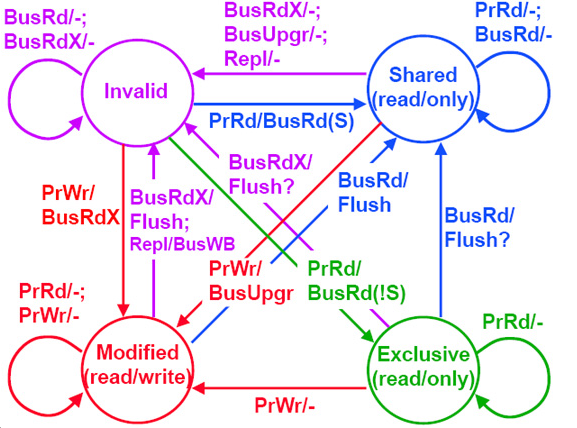
\includegraphics{mesi.xbb}
%\end{figure}
%% Store performance for a first write is poor.
%% \subsubsection{Store Buffers}
%% Added between CPU and cache
%% \subsubsection{Store Forwarding}
%% \subsubsection{Store Buffers and Memory Barriers}


\subsection{Summary and Acknowledgment}

Lot of the text is adaptation of Chapter 5 of Linux Kernel Programming
by Bovett and the memory barrier documentation part of the Linux
kernel by David Howells and Paul E. McKenney. Any errors are entirely
my own. For people looking for definitive and trustworthy accounts
looking at these sources is recommended.

\begin{thebibliography}{9}

\bibitem{ia32-sys}
  \textit{IA-32 Intel Architecture Software Developer's Manual, Volume 3:
    System Programming Guide} \\
  \textit{Chapter 7.1: Locked Atomic Operations} \\
  \textit{Chapter 7.2: Memory Ordering}  \\
  \textit{Chapter 7.4: Serializing Instructions}

\bibitem{unix-ma}
  \textit{Unix Systems for Modern Architectures, Symmetric Multiprocessing and Caching
    for Kernel Programmers} \\
  \textit{Chapter 13: Other Memory Models}  
  
\bibitem{mesi-wikipedia} 
  \textit{MESI protocol}  \\
  \url{http://en.wikipedia.org/wiki/MESI_protocol}
\bibitem{cache-coherency-primer} 
  \textit{Cache Coherency Primer}  \textit{Fabian "ryg" Giesen} \\
  \url{https://fgiesen.wordpress.com/2014/07/07/cache-coherency/}
 \bibitem{atomic-operations}
   \textit{Atomic Operations - CSE 378 University of Washington} \\
  \url{http://courses.cs.washington.edu/courses/cse378/07au/lectures/L25-Atomic-Operations.pdf}
\bibitem{memory-barriers}
  \textit{Linux Kernel Memory Barriers} \\
  \url{https://www.kernel.org/doc/Documentation/memory-barriers.txt}

\bibitem{atomic-operations}
  \textit{Semantics and Behavior of Atomic and Bitmask Operations} \\
  \textit{David S. Miller} \\
  \url{https://www.kernel.org/doc/Documentation/atomic_ops.txt}

\bibitem{columbia-sync-linux}
  \textit{Synchronization in Linux} \\
  \url{http://www.cs.columbia.edu/~junfeng/10sp-w4118/lectures/l11-synch-linux.pdf}

\bibitem{under-linux-kernel-sync}
  \textit{Understanding the Linux Kernel - Chapter 5} \\
  \textit{David Bovet and Marco Cesati}  

\bibitem{sadc}  
  \textit{Structures and Design of Computers } \\
  \textit{David E. Patterson and J.L. Hennessey} 
  
\bibitem{whymem}
  \textit{Why memory barriers?} \\
  \textit{Paul McKay} \\
  \url{http://www.rdrop.com/users/paulmck/scalability/paper/whymb.2010.06.07c.pdf}
\end{thebibliography}

\end{document}
